\section{\label{sec:clas.beam}Beam Measuring and Monitoring}

There are several beam monitoring stations inside Hall \desg{B} before and after the \abbr{CLAS} detector. Most of these are used by the accelerator group to steer the beam to the target as they control all magnets that can substantially move the beam. Other devices are used to measure the position, flux and dispersion of the beam. Upstream of \abbr{CLAS} there are two beam position monitors (\abbr{BPM}s\label{abbr:bpm}) placed before the tagger. These are used to measure the transverse location of the electron beam and its intensity. This information is used as feed back for the steering mechanism.

There are also two \emph{harp} devices located before the tagger that are used to measure the size of the electron beam; such a measurement for \g12 is shown in Fig.~\ref{fig:clas.beam.harpscan}. The harp devices consist of fine wires (20 and 50~{\um} W and 100~{\um} Fe) that pass through the beam at specific orientations to obtain a horizontal ($x$) and vertical ($y$) profile. Since this process is invasive, it was only done when the drift-chambers and \abbr{DAQ} were turned off.

\begin{figure}\begin{center}
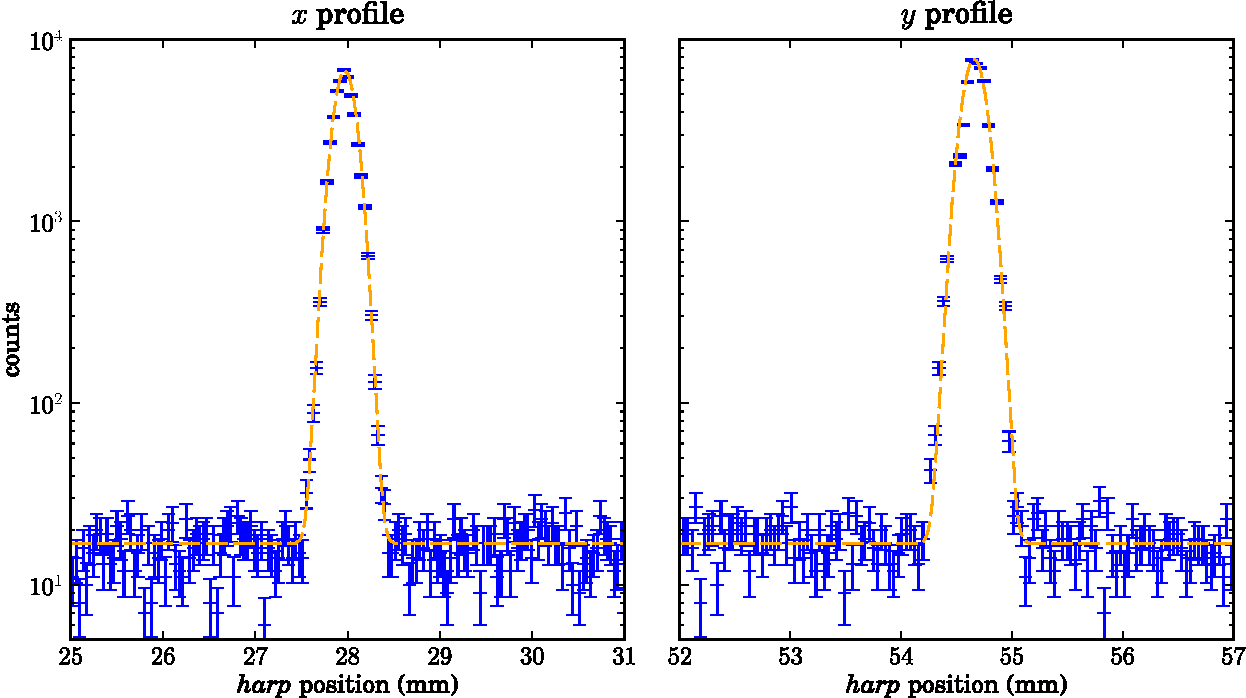
\includegraphics[width=\figwidth]{\grpath/calibration/harpscan.pdf}
\caption[Example \emph{harp} Scan for \g12]{\label{fig:clas.beam.harpscan}{\coloronline}A typical \emph{harp} scan done just prior to run 56426. Shown are the $x$ and $y$ profiles of the electron beam just before the tagger. The dashed orange line is a Gaussian fit to the data: $\sigma_x~=~0.115$~mm and $\sigma_y~=~0.105$~mm.}
\end{center}\end{figure}

A few meters downstream of the target is the Total Absorption Shower Counter (\abbr{TASC}\label{abbr:tasc}) which is used to measure the photon flux. The \abbr{TASC}, consists of four lead glass blocks, covering the entire beam, each instrumented by a photo-multiplier tube (\abbr{PMT}\label{abbr:pmt}) and having approximately 100\% photon detection efficiency at beam currents less than 100~pA\cite{clas.tagger,clas.tagger.calib}. Using these counters, \emph{normalization runs} of low current (50~pA, see Table~\ref{tab:data.calibruns}) were taken several times throughout \g12. In this way, the tagger was calibrated to measure the flux for the entire run period.
